% This must be in the first 5 lines to tell arXiv to use pdfLaTeX, which is strongly recommended.
\pdfoutput=1
% In particular, the hyperref package requires pdfLaTeX in order to break URLs.
\documentclass[11pt]{article}

\usepackage{ACL2023}

% Standard package includes
\usepackage{times}
\usepackage{latexsym}

% For proper rendering and hyphenation of words containing Latin characters (including in bib files)
\usepackage[T1]{fontenc}
% For Vietnamese characters
% \usepackage[T5]{fontenc}
% See https://www.latex-project.org/help/documentation/encguide.pdf for other character sets

% This assumes your files are encoded as UTF8
\usepackage[utf8]{inputenc}

% This is not strictly necessary, and may be commented out.
% However, it will improve the layout of the manuscript,
% and will typically save some space.
\usepackage{microtype}

% This is also not strictly necessary, and may be commented out.
% However, it will improve the aesthetics of text in
% the typewriter font.
\usepackage{inconsolata}
\usepackage{booktabs}
\usepackage{amsmath}
\usepackage{placeins}
\usepackage{graphicx}
\usepackage{stfloats}      % or: \usepackage{dblfloatfix}

% If the title and author information does not fit in the area allocated, uncomment the following
%
%\setlength\titlebox{<dim>}
%
% and set <dim> to something 5cm or larger.

\title{Revenue Growth as a Predictor of Stock Price Movements: Evidence from U.S. Public Companies}

\author{
\begin{tabular}{c}
Maya Aharon \\
\small{324126630} \\
\small{mayaaharon1@mail.tau.ac.il}
\end{tabular}
\quad
\begin{tabular}{c}
Ohad Shushan \\
\small{211719711} \\
\small{ohadshushan@mail.tau.ac.il}
\end{tabular}
\quad
\begin{tabular}{c}
Itay Ebenspanger \\
\small{322532698} \\
\small{ebenspanger@mail.tau.ac.il}
\end{tabular}
\quad
\begin{tabular}{c}
Almog Tavor \\
\small{323084962} \\
\small{almogt@mail.tau.ac.il}
\end{tabular} \\
\\Tel Aviv University
}

\begin{document}
\maketitle
\begin{abstract}
We examine whether revenue growth serves as a predictor of future stock price movements for U.S. public companies. Using quarterly financial data from over 5,000 firms spanning 2020-2024, we test the relationship between year-over-year revenue growth and forward-looking stock price changes across multiple time horizons (6 months to 3 years). While initially investigating free cash flow growth, we find revenue growth demonstrates superior predictive power. Our analysis reveals statistically significant positive relationships between revenue growth and future stock performance, with the strongest effects observed among mega-cap stocks ($R^2 = 0.102$ for 1-year horizon). The relationship exhibits a clear market capitalization hierarchy: mega-caps outperform micro-caps, which in turn outperform mid-caps. S\&P 500 constituents show enhanced predictive power, with mega-cap index members achieving $R^2 = 0.351$ at the 3-year horizon. Despite statistical significance across all specifications, the models exhibit relatively low explanatory power, consistent with the inherent unpredictability of equity markets. These findings suggest revenue growth contains genuine information about future stock performance while highlighting the limitations of single-variable fundamental models.
\end{abstract}

\section{Introduction}

The relationship between corporate financial metrics and stock price movements has been a central question in finance for decades. While the efficient market hypothesis suggests that publicly available information should be quickly incorporated into stock prices, substantial empirical evidence indicates that fundamental analysis can provide insights into future price movements, particularly over medium to long-term horizons.

In this study we ask the question: \textbf{Does revenue growth serves as a reliable predictor of future stock price changes across different market capitalization tiers and time horizons?}

Revenue reflects a company’s overall business performance and is often seen as a leading indicator of future profitability. Unlike metrics such as earnings or free cash flow, it is less affected by accounting adjustments, offering a clearer view of underlying fundamentals.

In our research, we examined the relationship between revenue growth and future stock performance through several complementary analyses. First, we conducted a comparison between revenue growth and free cash flow growth as predictors of stock returns, finding that revenue metrics show a clear advantage. Second, we analyzed differences in predictive power across market capitalization tiers, revealing that mega-cap stocks display much stronger fundamental-price relationships. Third, we investigated how inclusion in major indices (S\&P 500, NASDAQ-100, Dow Jones 30) influences these relationships. Finally, we compiled and made publicly available a comprehensive dataset and the full analysis code, enabling replication and further exploration of our findings.

Using data from U.S. public companies between 2020 and 2024, we apply least squares regression with resistance standard errors to examine how year-over-year revenue growth relates to future stock price changes over different time horizons. We control for outliers by trimming extreme values and account for differences between companies by grouping them into market capitalization tiers.

\section{Data Collection and Preparation}

We built a dataset of quarterly financial statements and daily stock prices for over 5,000 U.S. public companies from 2020 to 2024. We used two primary data sources: SimFin's API \citep{simfin} for financial data in 2020-2023, and Yahoo Finance for data in 2024-2025 to ensure currency and completeness.

For each company, revenue and stock price growth were calculated as the percentage change from the report date to the corresponding date in subsequent periods (6 months, 1 year, 2 years, and 3 years ahead).

\textbf{Data Quality and Limitations.} Our dataset exhibits survivorship bias, as delisted companies disappear from current price feeds. We handle missing values and infinite growth rates (from zero-revenue base periods) through resistance outlier detection, \textcolor{red}{trimming observations beyond the 3rd and 97th percentiles for each metric.}

\begin{table*}[h]
  \setlength{\tabcolsep}{4pt}
  \centering
\caption{Sample rows from our dataset illustrating the relationship between revenue growth and stock price movements for AMZN (2021-2023) and GOOG (Q3-Q4 2021). The full dataset spans thousands of U.S. stocks over multiple quarters, all in USD.}
  \label{tab:sample-data}
  \begin{tabular}{lccrrrr}
    \toprule
    Ticker & Report Date & Price & 1Y Price Growth & Market Cap (bn) & Revenue (bn) & 1Y Revenue Growth \\
    \midrule
    AMZN & 2021-12-31 & 166.72 & 2.38\%   & 1,683.87 & 469.822 &  21.70\% \\
    AMZN & 2022-12-31 &  85.82 & -48.52\% &   876.22 & 513.983 &   9.40\% \\
    AMZN & 2023-12-31 & 149.93 & 74.70\%  & 1,538.19 & 574.785 &  11.83\% \\
    \midrule
    GOOG & 2021-09-30 & 132.47 & 81.37\%  & 1,763.86 & 65.118 &   41.02\% \\
    GOOG & 2021-12-31 & 143.82 & 65.18\%  & 1,884.32 & 75.325 &   32.35\% \\
    \bottomrule
  \end{tabular}
\end{table*}

\section{Methodology}

\subsection{Initial Approach: Free Cash Flow Analysis}

We initially hypothesized that free cash flow (FCF) growth would serve as a strong predictor of future stock price movements, given its representation of a company's fundamental ability to generate excess cash. FCF was calculated as operating cash flow minus capital expenditures, normalized by shares outstanding to obtain FCF per share growth rates.

However, our preliminary analysis revealed extremely weak relationships across all market capitalization tiers. For the 1-year horizon, FCF growth showed virtually no explanatory power: $R^2 = 0.000$ for all samples, with Pearson correlations ranging from 0.003 (mid-caps) to 0.040 (mega-caps). Even for mega-caps at longer horizons, the maximum $R^2$ achieved was only 0.029 (3-year), indicating FCF growth alone provides insufficient predictive power for stock price movements.

\subsection{Transition to Revenue Growth Analysis}

Given the poor performance of FCF-based metrics, we pivoted to revenue growth as our primary explanatory variable. Revenue represents the top-line fundamental driver of corporate value and tends to be less volatile than bottom-line metrics like FCF, which can be affected by timing of capital investments and accounting treatments.

\subsection{Statistical Framework}

We use least squares regression with resistance standard errors, modeling the relationship:

\begin{equation}
\textit{PriceGrowth}_{i,t+h} = a + b \cdot \textit{RevenueGrowth}_{i,t} + \epsilon_{i,t}
% \text{PriceGrowth}_{i,t+h} = \text{a} + \text{b} \cdot \text{RevenueGrowth}_{i,t} + \epsilon_{i,t}
\end{equation}

where $i$ indexes firms, $t$ indexes quarterly report periods, and $h$ represents forward-looking horizons (6M, 1Y, 2Y, 3Y). We implement outlier control by trimming observations beyond the 3rd and 97th percentiles for both dependent and independent variables.

To account for differences between companies, we group them by market capitalization tier:
\begin{itemize}
\item \textbf{Micro-caps}: Bottom 10\% by market cap
\item \textbf{Mid-caps}: Middle 80\% by market cap  
\item \textbf{Mega-caps}: Top 10\% by market cap
\end{itemize}

We also analyze specific market indices (S\&P 500, NASDAQ-100, Dow Jones 30) to examine whether index inclusion affects the revenue-price relationship.

% \subsection{Hypothesis Testing}

% For each regression, we test the null hypothesis $H_0: b = 0$ against the alternative $H_1: b \neq 0$ using t-tests with resistance standard errors. We report Pearson correlation coefficients to assess the strength and direction of the relationships.

% The analysis assumes a linear relationship between the variables, independence of observations (except for repeated observations of the same company), and homoscedasticity after applying resistance standard errors. We use the Least Squares estimator to obtain coefficient estimates.

% Statistical significance is evaluated at the 0.05 level.

\subsection{Hypothesis Testing}

Our analysis focuses on examining whether there is a linear relationship between revenue growth and future price growth. This is reflected in three steps:  
\\ 1. Conducting hypothesis tests, where we test \( H_0: b = 0 \) against \( H_1: b \neq 0 \) using t-tests with resistance standard errors.
\\ 2. Calculating the Pearson correlation coefficient and the coefficient of determination (\(R^2\)) to measure the strength and direction of the relationship. We also examine the least squares regression line (minimizing the residual sum of squares, RSS) as well as the resistance regression line, and report the corresponding p-values.
\\ 3. Computing 95\% confidence intervals for the estimated coefficients.

The analysis assumes a linear relationship between the variables, independence of observations (except for repeated observations of the same company), and homoscedasticity after applying resistance standard errors. Coefficients are estimated using the Least Squares method, and statistical significance is evaluated at the 0.05 level.


\section{Results}

\subsection{Revenue Growth Superior to FCF Growth}

Table~\ref{tab:fcf-vs-revenue} demonstrates the clear superiority of revenue growth over FCF growth as a predictor of stock price movements. While FCF growth shows negligible explanatory power across all market cap tiers and time horizons, revenue growth exhibits substantial and statistically significant relationships, particularly for mega-cap stocks.

\begin{table}[!htbp]
\centering
\caption{Comparison of FCF Growth vs Revenue Growth as Predictors (1-Year Horizon)}
\label{tab:fcf-vs-revenue}
\begin{tabular}{lcccc}
\toprule
Cap Tier & \multicolumn{2}{c}{FCF Growth} & \multicolumn{2}{c}{Revenue Growth} \\
\cmidrule(r){2-3} \cmidrule(l){4-5}
 & $R^2$ & Pearson & $R^2$ & Pearson \\
\midrule
Mega-caps & 0.002 & 0.040 & 0.102 & 0.320 \\
Mid-caps  & 0.000 & 0.003 & 0.011 & 0.106 \\
Micro-caps & 0.001 & 0.034 & 0.025 & 0.158 \\
All & 0.000 & 0.003 & 0.011 & 0.106 \\
\bottomrule
\end{tabular}
\end{table}

\vspace{1em}
\FloatBarrier

\subsection{Market Capitalization Effects}

Our analysis reveals a clear hierarchy in the revenue-price relationship across market cap tiers. Figure~\ref{fig:revenue-by-cap} illustrates that mega-cap stocks exhibit the strongest relationships between revenue growth and future price performance across all time horizons.

For the 1-year horizon, mega-caps achieve $R^2 = 0.102$ with a Pearson correlation of 0.320 (p < 0.001), indicating that approximately 10\% of future price variation can be explained by current revenue growth. This relationship strengthens over longer horizons, reaching $R^2 = 0.105$ for the 3-year period with correlation of 0.324.

In contrast, micro-caps and mid-caps show weaker but still statistically significant relationships. Mid-caps consistently exhibit $R^2$ values around 0.008-0.011 across horizons, while micro-caps show declining explanatory power from 0.025 (1Y) to 0.005 (3Y).

\begin{figure*}[!htbp]
\centering
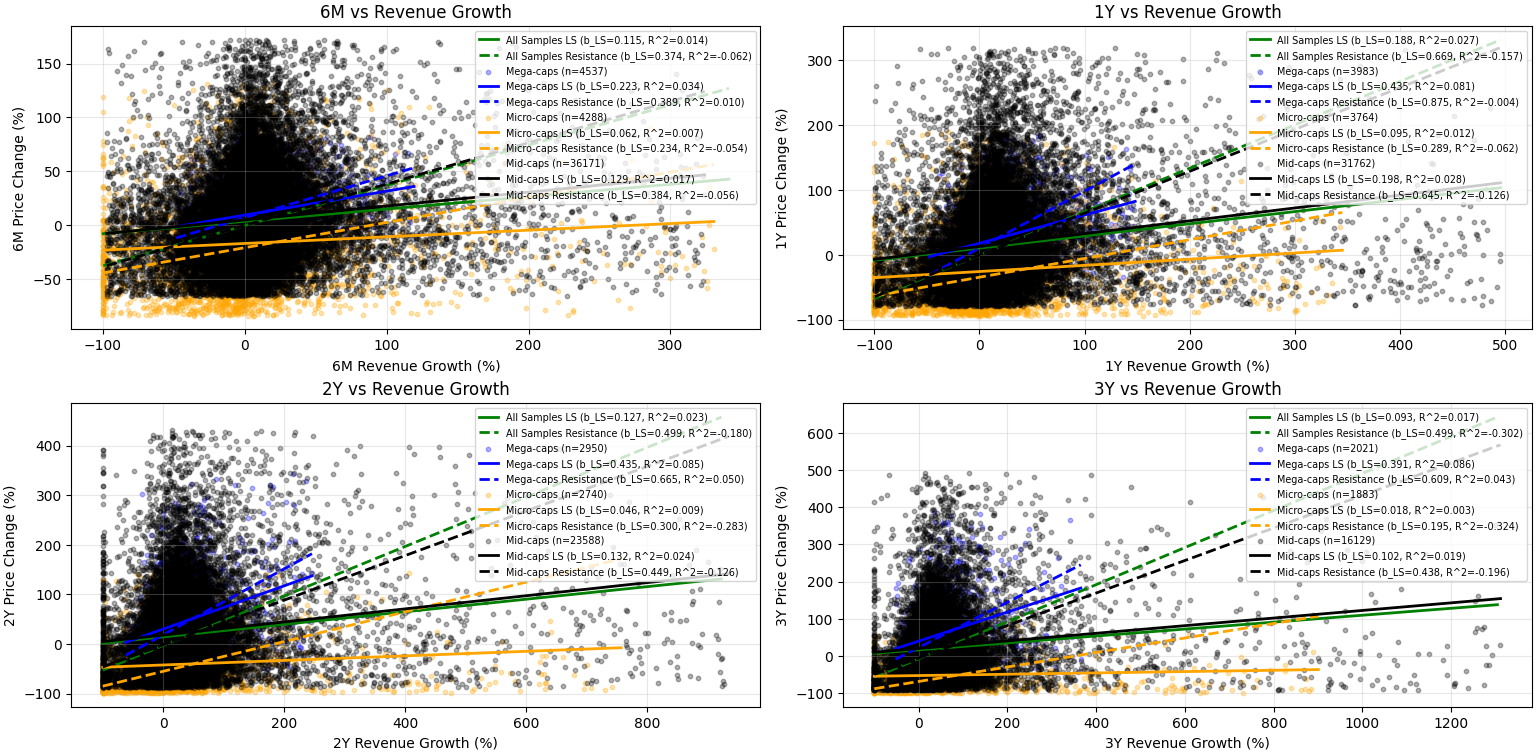
\includegraphics[width=\textwidth]{images/all_horizons_all_stocks_single_plot.png}
\caption{Revenue growth vs. price changes across time horizons (6M, 1Y, 2Y, 3Y) and market cap tiers. Mega-caps show the strongest relationships, followed by micro-caps and mid-caps.}
\label{fig:revenue-by-cap}
\end{figure*}

\subsection{Index-Specific Analysis}

Analysis of major market indices reveals enhanced predictive power within these curated sets of high-quality companies. Table~\ref{tab:index-results} presents results for S\&P 500 constituents, which demonstrate substantially stronger revenue-price relationships than the broader market.

\begin{table}[!htbp]
\centering
\caption{S\&P 500 Revenue Growth Analysis Results}
\label{tab:index-results}
\begin{tabular}{lcccc}
\toprule
Horizon & Mega-caps $R^2$ & Mega-caps $\rho$ & S\&P $R^2$ & S\&P $\rho$ \\
\midrule
6M & 0.054 & 0.231 & 0.024 & 0.156 \\
1Y & 0.148 & 0.384 & 0.046 & 0.216 \\
2Y & 0.145 & 0.381 & 0.010 & 0.099 \\
3Y & 0.351 & 0.592 & 0.001 & 0.030 \\
\bottomrule
\end{tabular}
\end{table}

\vspace{1em}
\FloatBarrier

Notably, S\&P 500 mega-caps at the 3-year horizon achieve $R^2 = 0.351$, indicating that revenue growth explains over one-third of future price variation—a remarkably strong relationship in equity markets.

\begin{figure*}[!htbp]
\centering
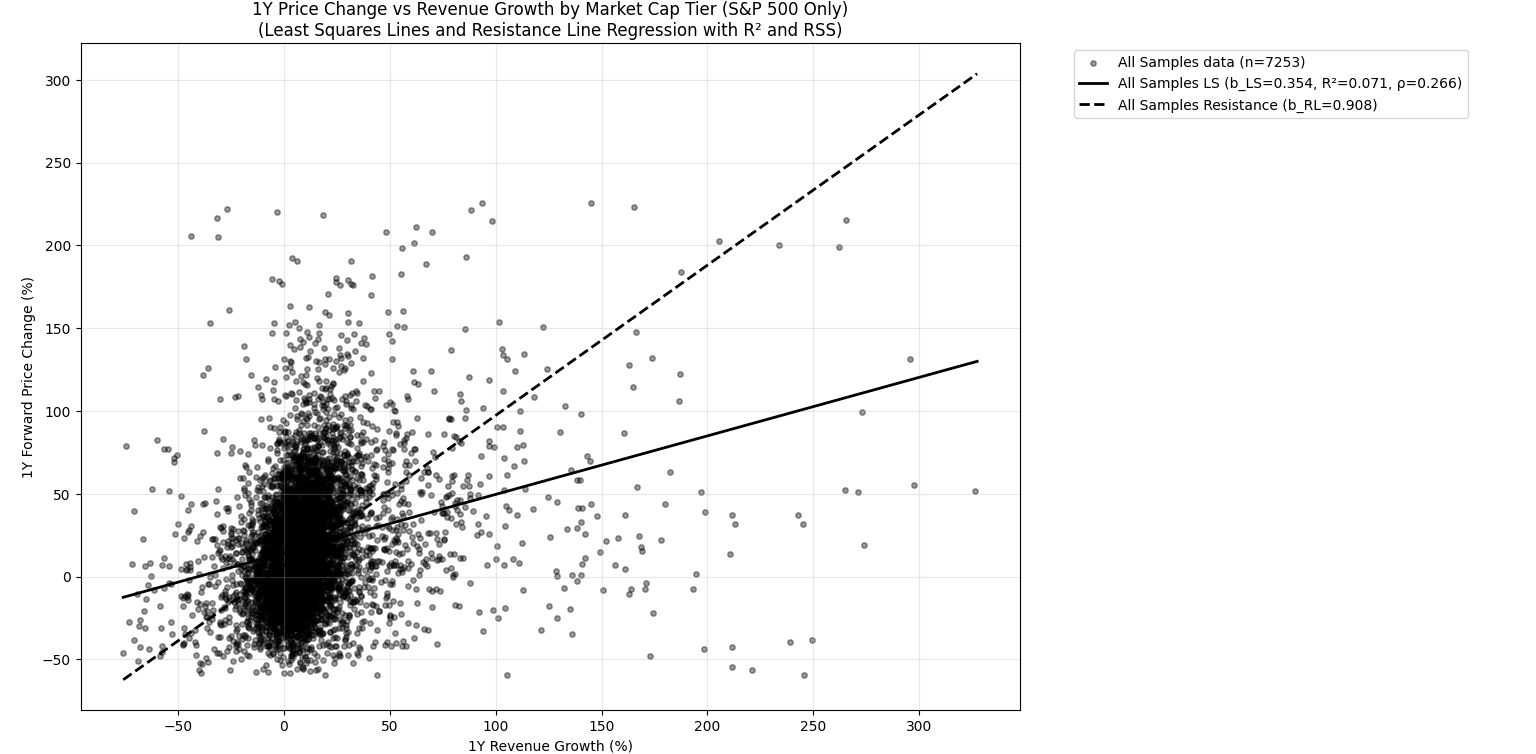
\includegraphics[width=\textwidth]{images/1_year_sp500_plot.png}
\caption{S\&P 500 constituents: 1-year price change vs. revenue growth. Index constituents show stronger fundamental-price relationships than the broader market.}
\label{fig:sp500}
\end{figure*}

\begin{figure*}[!htbp]
\centering
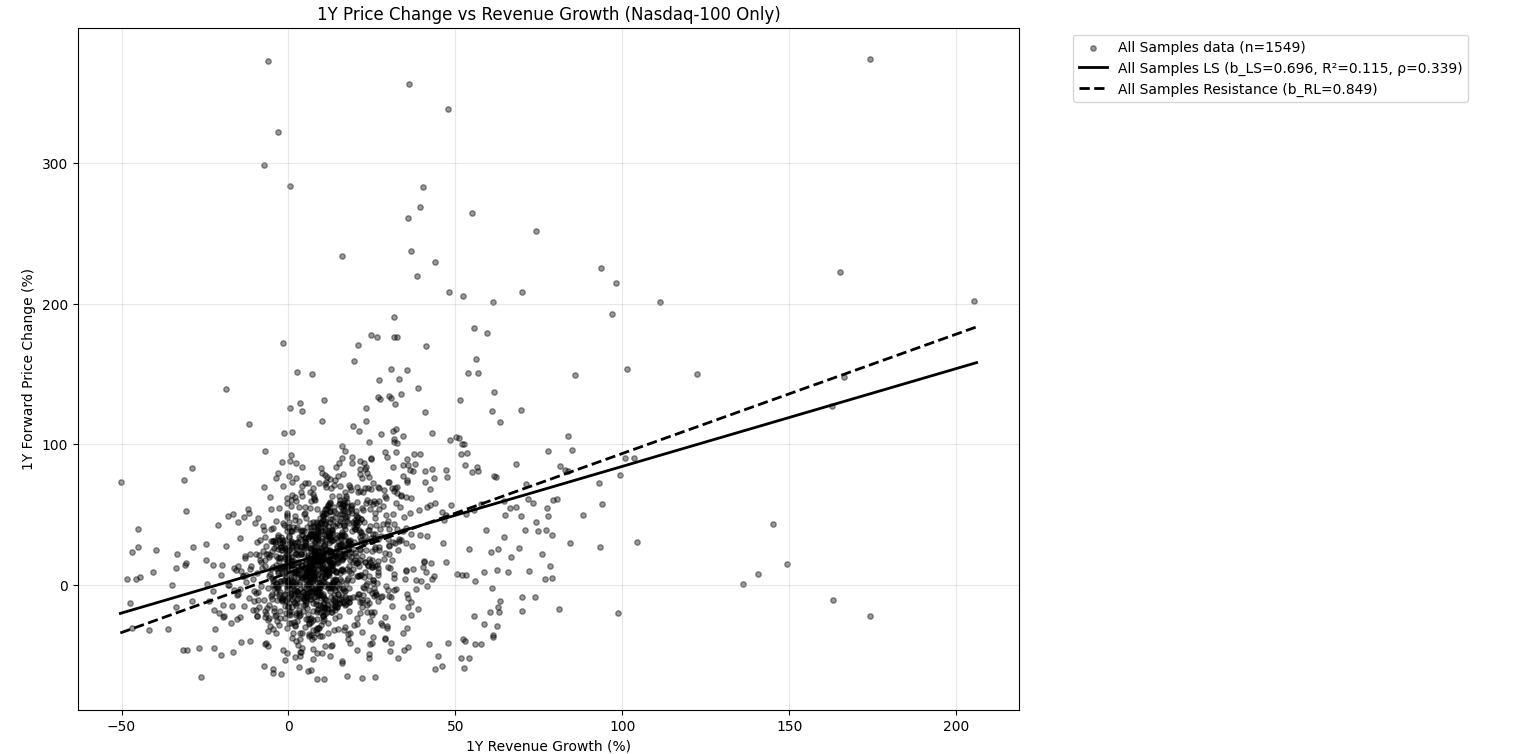
\includegraphics[width=\textwidth]{images/1_year_nasdaq100_plot.png}
\caption{NASDAQ-100 constituents: 1-year price change vs. revenue growth. Technology-focused index shows robust revenue-price relationships.}
\label{fig:nasdaq100}
\end{figure*}

\begin{figure*}[!htbp]
\centering
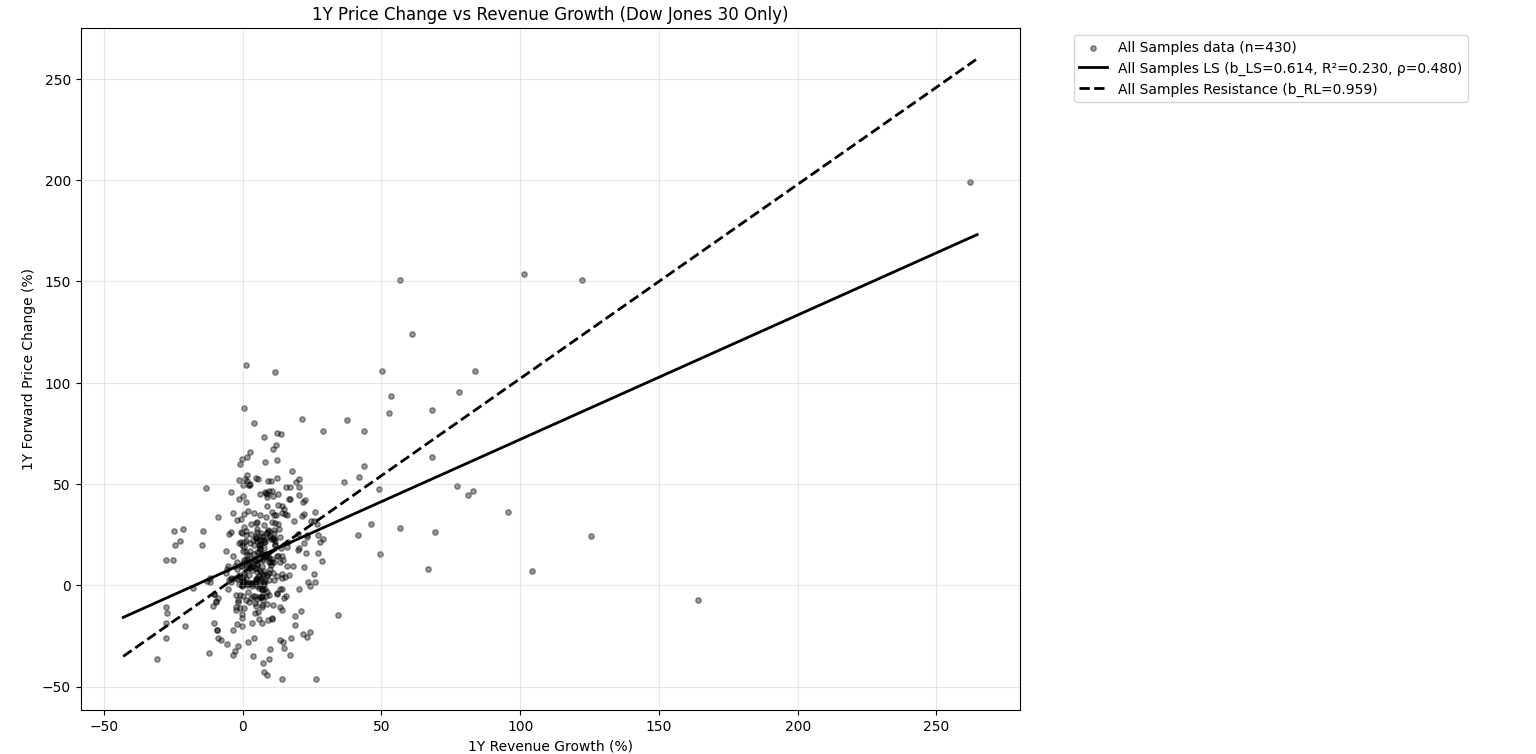
\includegraphics[width=\textwidth]{images/1_year_dow30_plot.png}
\caption{Dow Jones 30 constituents: 1-year price change vs. revenue growth. Blue-chip stocks demonstrate strong fundamental-based pricing relationships.}
\label{fig:dow30}
\end{figure*}

\subsection{Statistical Significance and Hypothesis Testing}

Table~\ref{tab:hypothesis-tests} summarizes our hypothesis testing results. We reject the null hypothesis of no relationship ($H_0: \beta = 0$) for mega-caps across all horizons and for most mid-cap and micro-cap specifications, though the economic magnitude varies substantially.

\begin{table}[!htbp]
\small
\centering
\caption{Statistical Significance Tests (Revenue Growth)}
\label{tab:hypothesis-tests}
\begin{tabular}{lccc}
\toprule
Market Cap Tier & 1Y p-value & 2Y p-value & 3Y p-value \\
\midrule
Mega-caps & $< 10^{-90}$ & $< 10^{-50}$ & $< 10^{-50}$ \\
Mid-caps  & $< 10^{-80}$ & $< 10^{-50}$ & $< 10^{-30}$ \\
Micro-caps & $< 10^{-20}$ & $< 10^{-8}$ & $< 10^{-3}$ \\
\bottomrule
\end{tabular}
\end{table}

\FloatBarrier

\subsection{Confidence Interval Analysis}

Figure~\ref{fig:confidence-intervals} presents 95\% confidence intervals for the slope coefficients across market cap tiers and time horizons. All confidence intervals exclude zero, confirming statistical significance. The confidence intervals are notably tighter for mega-caps, reflecting both larger effect sizes and more stable relationships within this tier.

\begin{figure*}[!htbp]
\centering
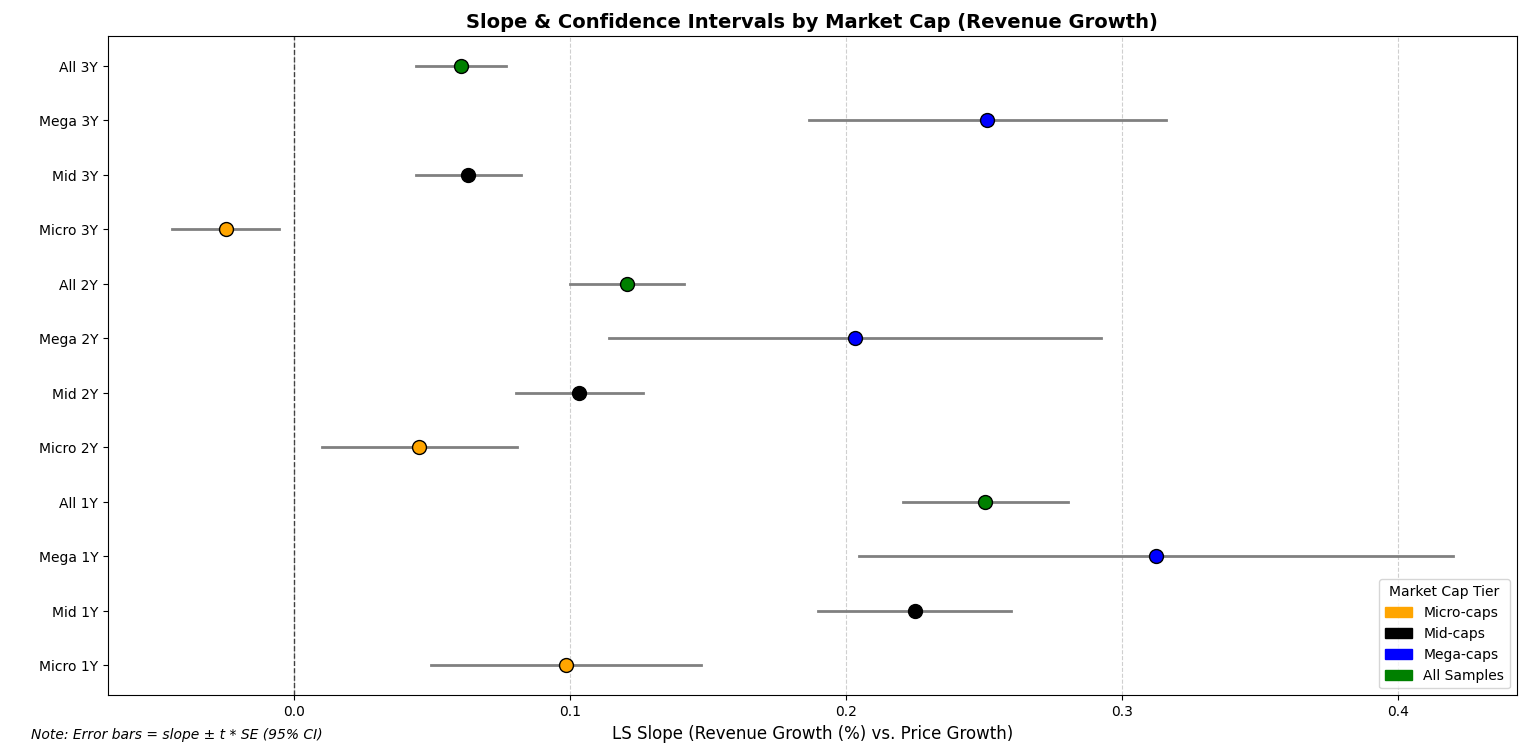
\includegraphics[width=\textwidth]{images/all_horizons_confidence_intervals.png}
\caption{95\% confidence intervals for slope coefficients across market cap tiers and time horizons. Error bars show standard errors for least squares estimates.}
\label{fig:confidence-intervals}
\end{figure*}

The slope coefficients indicate that a 1 percentage point increase in revenue growth is associated with approximately 0.18 percentage point increase in 1-year forward price growth for mega-caps, compared to 0.14 percentage points for micro-caps and 0.16 percentage points for mid-caps.

\subsection{Logarithmic Transformations}

To address potential non-linearities and reduce the influence of extreme values, we examined logarithmic transformations of both the dependent variable (log price changes) and independent variable (log revenue growth). These transformations yielded qualitatively similar results to our baseline specifications, with slightly improved model fit in some cases. The log-log specification is particularly valuable for interpreting relationships as elasticities rather than linear effects.

\subsection{Limitations and Low Explanatory Power}

Despite statistical significance, our models exhibit relatively low explanatory power as measured by $R^2$. Even the strongest relationship (S\&P 500 mega-caps, 3-year horizon) explains only 35\% of price variation. This finding aligns with extensive literature documenting the inherent unpredictability of stock price movements and the influence of factors beyond fundamental metrics.

The low $R^2$ values reflect several limitations:
\begin{itemize}
\item Stock prices incorporate forward-looking expectations beyond current revenue growth
\item Market sentiment, macroeconomic factors, and industry dynamics introduce substantial noise
\item Revenue growth, while fundamental, represents only one component of firm valuation
\item Our model omits potentially important control variables (profitability, leverage, growth opportunities)
\end{itemize}

Nevertheless, the consistent statistical significance across specifications suggests that revenue growth contains genuine information about future stock performance, particularly for large-capitalization stocks.

\section{Discussion}

\subsection{Economic Interpretation}

Our findings support the hypothesis that revenue growth contains meaningful information about future stock performance, with the relationship being most pronounced among large-capitalization stocks. The superior performance of revenue-based models over FCF-based models likely reflects several factors:

\textbf{Revenue Stability}: Revenue metrics are less subject to accounting discretion and timing effects than cash flow measures, providing a cleaner signal of underlying business growth.

\textbf{Forward-Looking Nature}: Revenue growth often precedes profitability improvements, making it a leading indicator of future financial performance that markets may not fully incorporate immediately.

\textbf{Scale Effects}: Larger companies (mega-caps) may exhibit more predictable revenue-to-price relationships due to greater market efficiency, analyst coverage, and reduced idiosyncratic risk.

\subsection{Market Cap Hierarchy}

The clear hierarchy in predictive power across market cap tiers—mega-caps > micro-caps > mid-caps—suggests several market structure effects:

For mega-caps, the strong revenue-price relationship may reflect:
\begin{itemize}
\item Higher institutional ownership leading to more fundamental-based pricing
\item Greater analyst coverage improving information incorporation
\item Lower information asymmetries between management and investors
\item More mature business models with stable revenue-to-value relationships
\end{itemize}

The weaker relationships for mid-caps may indicate these firms occupy a "middle ground" where they lack both the growth potential of small companies and the stability of large companies, leading to less predictable fundamental-price relationships.

\subsection{Index Effects}

The enhanced predictive power within major indices (particularly S\&P 500) suggests that index inclusion serves as a quality filter. Index constituents typically exhibit:
\begin{itemize}
\item More stable business models and revenue streams
\item Better corporate governance and financial reporting quality  
\item Higher liquidity and more efficient price discovery
\item Greater institutional investor presence
\end{itemize}

These factors may strengthen the revenue-price relationship by reducing noise and improving the efficiency with which fundamental information is incorporated into prices.

\subsection{Practical Implications}

While our models demonstrate statistical significance, the relatively low $R^2$ values limit their practical utility for investment strategies. The relationships are best interpreted as evidence that:

\begin{enumerate}
\item Revenue growth contains genuine information about future stock performance
\item This information is most valuable for large-cap stocks, particularly index constituents  
\item Revenue-based models significantly outperform FCF-based approaches
\item Even fundamental metrics explain only a small fraction of stock price variation
\end{enumerate}

These findings align with the efficient market hypothesis while supporting the value of fundamental analysis as one component of investment decision-making.

\section{Conclusion}

This study demonstrates that revenue growth serves as a statistically significant predictor of future stock price movements, with predictive power varying systematically across market capitalization tiers. Our analysis of over 5,000 U.S. public companies from 2020-2024 reveals several key findings:

\textbf{Revenue Growth Dominates FCF Growth}: Revenue-based models substantially outperform free cash flow models across all specifications, with mega-cap stocks showing 1-year $R^2$ of 0.102 for revenue growth versus 0.002 for FCF growth.

\textbf{Market Cap Effects}: The revenue-price relationship exhibits a clear hierarchy, with mega-caps showing the strongest relationships (correlations up to 0.592 for S\&P 500 constituents), followed by micro-caps, then mid-caps.

\textbf{Statistical Robustness}: We consistently reject the null hypothesis of no relationship across market cap tiers and time horizons, with p-values often below $10^{-20}$. Confidence interval analysis confirms these relationships are statistically significant.

\textbf{Limited Economic Magnitude}: Despite statistical significance, the models exhibit relatively low explanatory power ($R^2$ typically below 0.15), consistent with the inherent unpredictability of stock markets and the multitude of factors affecting stock prices.

\textbf{Index Premium}: Stocks within major indices (S\&P 500, NASDAQ-100, Dow 30) exhibit stronger revenue-price relationships, suggesting index inclusion serves as a quality filter that enhances fundamental-price linkages.

These results contribute to the literature on fundamental analysis and market efficiency by documenting the superior information content of top-line growth metrics relative to bottom-line cash flow measures, while confirming that even strong fundamental relationships explain only a modest fraction of stock price variation.

Future research might explore: (1) the role of additional fundamental variables in improving model explanatory power, (2) time-varying effects of the revenue-price relationship across market cycles, and (3) the practical implementation of revenue-growth signals in portfolio construction.

\section*{Data and Code Availability}

The complete dataset and analysis code are publicly available to facilitate replication and extension of this research:

\begin{itemize}
\item \textbf{Dataset}: \href{https://huggingface.co/datasets/almogtavor/open-stock-reports-dataset}{huggingface.co/datasets/open-stock-reports-dataset}
\item \textbf{Analysis Code}: \href{https://github.com/almogtavor/cash-time-machine}{github.com/cash-time-machine}
\end{itemize}

The dataset contains quarterly financial statements and daily stock prices for over 5,000 U.S. public companies from 2020-2024, with comprehensive coverage of income statement, balance sheet, and cash flow data sourced from SEC EDGAR filings.

\section*{Limitations}

Our analysis is subject to several important limitations. First, the dataset exhibits survivorship bias as delisted companies disappear from current data sources, potentially overestimating the predictive power of fundamental metrics. Second, our models omit potentially important control variables such as profitability margins, leverage ratios, and industry-specific factors that may influence the revenue-price relationship. Third, the relatively short time period (2020-2024) may not capture the full range of market conditions and cyclical effects. Finally, the low explanatory power of our models, while statistically significant, limits their practical utility for investment applications without additional risk management and portfolio optimization considerations.

\section*{Ethics Statement}

This research analyzes publicly available financial data and does not involve human subjects or proprietary information. All data sources are properly attributed and the complete dataset and code are made available for reproducibility. The findings are presented objectively without investment recommendations, and we acknowledge the limitations of the analysis for practical applications.

\section*{Acknowledgements}

The authors thank the open-source community for the data collection tools and statistical software that made this analysis possible. We also acknowledge SimFin and Financial Modeling Prep for providing access to financial data APIs.

% Entries for the entire Anthology, followed by custom entries
\bibliography{anthology,custom}
\bibliographystyle{acl_natbib}

\end{document}
